\section{Planning and Time Management}
\begin{figure}[H]
	\centering
	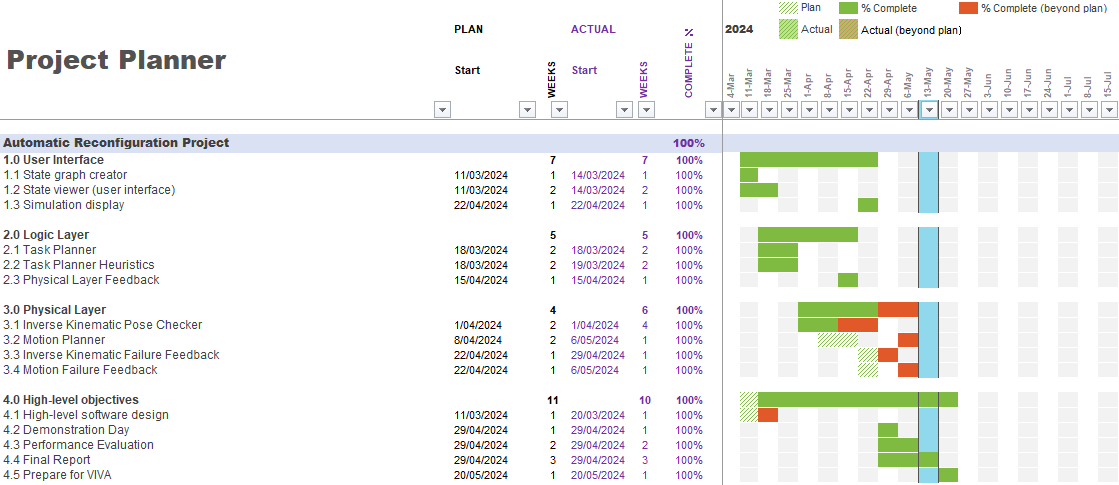
\includegraphics[width=\textwidth]{projectPlanner.png}
	\caption{Project Plan after project completion. Task descriptions can be seen in \nameref{Initial Report}}
	\label{planner}
\end{figure}
\subsection{Project Management Procedures}
To streamline the design and development of the project, it followed a traditional engineering product development cycle consisting of 5 phases:
\begin{itemize}[]
	\item\textbf{Initiation:} The definition of the problem and the projects goals, requirements, and risks. This phase was completed by the given description of the project and further questioning of the project supervisor.
	\item\textbf{Planning:} The definition of how to solve the problem by outlining the details and goals to meet the defined requirements. This phase was completed by the production of the initial report seen in \nameref{Initial Report}, the project plan seen in figure \ref{planner}, and a conceptual high-level product design. 
	\item\textbf{Execution:} The working phase where the plan designed in the previous phase is put into action and the product is developed. This was completed according to the created project plan and was finished in its majority by the project demonstration day on the 29th of April 2024.
	\item\textbf{Controlling \& Monitoring:} This phase runs alongside the execution phase and involves tracking progress and adjusting the workflow to remove potential roadblocks.
	\item\textbf{Closure:} Reflecting on the progress and results to officially end the project. This phase is conducted through analysis of project results, documentation of completed work and reflection of project success which is represented by this document.
\end{itemize}

\subsection{Project Management Reflection}
The project went according to plan through to the development of the physical layer. Due to unfamiliarity with robot kinematics, little in-depth design was created in the planning phase of the project with the assumption that with the knowledge of what each section of the physical layer needed to accomplish, figuring out how to accomplish it would not be a notable obstacle. This led to the physical layers’ development taking far longer than expected, over-running its planned development time by a week despite completing the logic layer earlier than expected. Due to overrunning the deadline, the project goal was instead completed by defining a simple physical layer rule to use for feedback such as “is the module at the top of the stack and hence, can be picked up in an environment with gravity by a stationary arm”; allowing the remainder of the project to be completed, making it possible to develop and analyse feedback strategies without sacrificing time to develop a mostly unused and complex simulation.
\\\\ 
Despite the delay, the final product does match what was planned at the beginning of the project, and as such the goals of the project have been filled. This can be attributed to appropriate levels of slack in task timing guidelines and creatively making use of out-of-the-box implementations to decrease production time drastically and reduce complexity.

\subsection{Risk Assessment}
This section builds, and expands, on material previously included in the project Initial Report (see \nameref{Initial Report}).
\begin{figure}[H]
	\begin{tabularx}{\textwidth}{| >{\centering}p{0.03\textwidth} | p{0.25\textwidth} | >{\centering}p{0.08\textwidth} | p{0.25\textwidth} | X |}
		\hline
		\textbf{ID} & \textbf{Risk Description} & \textbf{Impact} & \textbf{Risk Mitigation} & \textbf{Effectiveness}\\
		\hline
		1 & Missing or corrupted documents & High & Documents are backed up to a GitHub \newline repository & Highly effective \\
		\hline
		2 & Ambitions for project are too great for the project time limit & High & Setting appropriate scope expectations from the beginning of the project & Slightly effective:\newline did not properly take into consideration prior knowledge \\
		\hline
		3 & Illness or work \newline unavailability & Medium & Record illness and \newline provide proper \newline explanation for missing work in final report. \newline Decrease scope to \newline provide meaningful\newline results & Highly effective:\newline Illness affected several weeks of the project; However, scope was reduced appropriately \\
		\hline
		4 & Losing test results & Medium & Produce lab reports to document progress & Highly effective \\
		\hline
	\end{tabularx}
	\caption{Project Risk Register}
	\label{riskRegister}
\end{figure}

\subsection{Evolution of Project Plan}
The project plan saw little modification over the project. During progress reviews during the project, if it was seen that a section of the project would overrun its deadline, alternative methods of reaching a functional overall system were found that involved sacrificing small features such as including module orientation and module connectivity direction. These features were still considered in the completed implementation allowing them to be designed and implemented with relative ease when the project is further developed in the future.